\documentclass[a4paper, 12pt]{article}
\usepackage[utf8x]{inputenc}
\usepackage[english, russian]{babel}
\usepackage[left=25mm, top=25mm, right=25mm, bottom=25mm]{geometry}
\usepackage{cmap}
\usepackage{indentfirst}
\usepackage{tikz}
\usepackage{float}
\usepackage{amsmath, amsfonts, amssymb}
\usepackage{graphicx}
\usepackage{hyperref}
\usepackage{listings}
\usepackage{caption}
\usepackage{subcaption}
\usepackage{xcolor}
\usepackage{etoolbox}
\usepackage{titlesec}
\pagestyle{plain}
\patchcmd{\tableofcontents}{\contentsname}{\centering\contentsname}{}{}
\titleformat{\section}[block]{\normalfont\large\bfseries\centering}{}{0pt}{}
\titleformat{\subsection}[block]{\normalfont\normalsize\bfseries\centering}{}{0pt}{}
\allowdisplaybreaks
\graphicspath{{src/images/}}
\usetikzlibrary{patterns}
\definecolor{LightGray}{gray}{0.95}
\definecolor{LightGray2}{gray}{0.7}
\lstdefinestyle{code}{
    language=MATLAB, % replace language here
    basicstyle=\footnotesize\ttfamily,
    % numbers=left,
    % numberstyle=\scriptsize\color{gray},
    % stepnumber=1,
    % numbersep=5pt,
    backgroundcolor=\color{LightGray},
    showspaces=false,
    showstringspaces=false,
    showtabs=false,
    tabsize=4,
    captionpos=b,
    breaklines=true,
    breakatwhitespace=false,
    frame=single,
    rulecolor=\color{LightGray2},
    linewidth=\linewidth,
    keywordstyle=\color{blue}\bfseries,
    commentstyle=\color{green!40!black},
    stringstyle=\color{purple},
    escapeinside={\%*}{*)},
    inputencoding=utf8x,
    xleftmargin=0pt,
    framexleftmargin=0pt,
    framexrightmargin=0pt
}
\lstset{style=code}
\hypersetup{
    colorlinks=true,
    linkcolor=blue,
    filecolor=magenta,
    urlcolor=cyan,
    pdftitle={contents setup},
    pdfpagemode=FullScreen,
}


\begin{document}
    \begin{titlepage}

        \begin{center}
        Федеральное государственное автономное образовательное учреждение высшего образования
        «Национальный Исследовательский Университет ИТМО»
        \vfill
        
        
\includegraphics[width=0.3\textwidth]{itmo.png} % requires /src/images/itmo.png

        {\large\bf ЛАБОРАТОРНАЯ РАБОТА №E}\\
        {\large\bf ПРЕДМЕТ «ТЕОРИЯ АВТОМАТИЧЕСКОГО УПРАВЛЕНИЯ»}\\
        {\large\bf ТЕМА «УПРАВЛЕНИЕ МНОГОКАНАЛЬНОЙ СИСТЕМОЙ»}\\
        Вариант №2
        \vfill

        \begin{flushright}
            \begin{minipage}{.45\textwidth}
            {
                \hbox{Преподаватель:}
                \hbox{Пашенко А. В.}
                \hbox{}
                \hbox{Выполнил:}
                \hbox{Румянцев А. А.}
                \hbox{}
                \hbox{Факультет: СУиР}
                \hbox{Группа: R3341}
                \hbox{Поток: ТАУ R22 бак 1.1.1}
            }
            \end{minipage}
        \end{flushright}
        \vfill
  
        Санкт-Петербург\\
        2025
        \end{center}
    \end{titlepage}
    
    \tableofcontents

    \newpage
    \section{Задание 1. Исследование свойств многоканальной системы}
    Рассмотрим многоканальную систему
    $$
    \begin{cases}
    \dot{x}=Ax+Bu,\\
    y=Cx,
    \end{cases} A=\begin{bmatrix}
        0 &1\\
        -1 &2
    \end{bmatrix},\ B=\begin{bmatrix}
        1 &2\\
        -3 &3
    \end{bmatrix},\ C=\begin{bmatrix}
        2 &1\\
        3 &-2
    \end{bmatrix},\ D=0;
    $$
    Программа для задания находится в приложении А на листинге \ref{task1}.


    \subsection{Собственные числа матрицы системы}
    Определим собственные числа $\lambda_i$ матрицы системы $A$
    $$
    \sigma\left[ A \right]=\left\{ 1,1 \right\}
    $$
    Получили кратные неустойчивые собственные числа.


    \subsection{Передаточная матрица многоканальной системы, ее нули и полюса}
    Определим передаточную матрицу многоканальной системы по формуле
    $$
    W(s)=C\left[ sI-A \right]^{-1}B+D
    $$
    Получаем
    $$
    W(s)=\begin{bmatrix}
        \dfrac{-s-11}{s^2-2s+1}	&\dfrac{7s-4}{s^2-2s+1}\\
        \dfrac{9s-13}{s^2-2s+1}	      &\dfrac{1}{s^2-2s+1}
    \end{bmatrix}
    $$
    Нули и полюса квадратной передаточной матрицы определяются из
    корней числителя и знаменателя определителя передаточной матрицы. Найдем определитель
    $$
    \det{\left[W(s)\right]}=\dfrac{-63}{s^2-2s+1}
    $$
    Так как числитель не зависит от $s$, то нули $n_i$ отсутствуют.
    Определим полюса $\lambda_i$
    $$
    s^2-2s+1=0,\ \left( s-1 \right)^2=0\Rightarrow \lambda_{1,2}=1
    $$
    Полюса совпали с собственными числами матрицы $A$.


    \subsection{Структурные свойства многоканальной системы}
    Структурные свойства многоканальной системы определяются таким
    же образом, как и для одноканальной. Найдем ЖНФ матрицы $A$,
    переведем $B,C$ в базис собственных векторов $A$
    $$
    J=\begin{bmatrix}
        1     &1\\
     0     &1
    \end{bmatrix},\ B_J=\begin{bmatrix}
        3    &-3\\
     4    &-1
    \end{bmatrix},\ C_J=\begin{bmatrix}
        -3     &2\\
    -1     &3
    \end{bmatrix};
    $$
    Также найдем матрицу управляемости по выходу и вычислим ее ранг
    $$
    U_{out}=\begin{bmatrix}
        CU &D
    \end{bmatrix},\ U=\begin{bmatrix}
        B &AB
    \end{bmatrix}\Rightarrow U_{out}=\begin{bmatrix}
        -1     &7   &-13    &10     &0     &0\\
     9     &0     &5     &1     &0     &0
    \end{bmatrix},\ \text{rank}\left[ U_{out} \right]=2;
    $$
    Таким образом,
    \begin{align*}
        &\circ \text{ Система полностью управляема по состоянию и стабилизируема}\\
        &\circ \text{ Система полностью наблюдаема и обнаруживаема}\\
        &\circ \text{ Система полностью управляема по выходу}
    \end{align*}


    \subsection{Временные характеристики системы}
    Для аналитического определения весовых функций воспользуемся
    обратным преобразованием Лапласа
    $$
    w_k(t)=\mathcal{L}^{-1}\left\{ W_{i,j}(s) \right\}
    $$
    Нам пригодятся эти формулы
    \begin{align}
        &\mathcal{L}^{-1}\left\{\dfrac{1}{\left( s-a \right)}\right\}=e^{at},\label{eq:help1} \\
        &\mathcal{L}^{-1}\left\{\dfrac{n!}{\left( s-a \right)^{n+1}}\right\}=t^ne^{at}; \label{eq:help2}
    \end{align}
    Выведем $w_1(t)$
    $$
    w_1(t)=\mathcal{L}^{-1}\left\{ W_{1,1}(s) \right\}=\mathcal{L}^{-1}\left\{ \dfrac{-s-11}{s^2-2s+1} \right\}
    $$
    Упростим передаточную функцию $W_{1,1}(s)$
    $$
    W_{1,1}(s)=\dfrac{-s-11}{s^2-2s+1}=-\dfrac{s-1+12}{\left( s-1 \right)^2}=-\dfrac{s-1}{\left( s-1 \right)^2}-\dfrac{12}{\left( s-1 \right)^2}=
    -1\cdot\dfrac{1}{\left(s-1\right)}-12\cdot\dfrac{1}{\left( s-1 \right)^2}
    $$
    Воспользуемся выражениями (\ref{eq:help1}), (\ref{eq:help2}) и свойствами линейности преобразования Лапласа и вычислим $w_1(t)$
    $$
    w_1(t)=\mathcal{L}^{-1}\left\{ -1\cdot\dfrac{1}{\left(s-1\right)}-12\cdot\dfrac{1}{\left( s-1 \right)^2} \right\}=
    -\mathcal{L}^{-1}\left\{ \dfrac{1}{\left(s-1\right)} \right\}-12\mathcal{L}^{-1}\left\{ \dfrac{1}{\left( s-1 \right)^2} \right\},
    $$
    $$
    w_1(t)=-e^t-12te^t;
    $$
    Найдем $w_2(t)$
    $$
    w_2(t)=\mathcal{L}^{-1}\left\{ W_{1,2} \right\}=\mathcal{L}^{-1}\left\{ \dfrac{7s-4}{\left( s-1 \right)^2} \right\}
    $$
    Упростим передаточную функцию $W_{1,2}(s)$
    $$
    W_{1,2}(s)=\dfrac{7s-4}{\left( s-1 \right)^2}=\dfrac{A}{\left(s-1\right)}+\dfrac{B}{\left( s-1 \right)^2}=\dfrac{As-A+B}{\left( s-1 \right)^2},
    $$
    $$
    As-A+B=7s-4\Rightarrow \begin{cases}
        A=7,\\
        -A+B=-4,
    \end{cases}\Rightarrow B=-4+A=-4+7=3,
    $$
    $$
    W_{1,2}(s)=\dfrac{7}{\left( s-1 \right)}+\dfrac{3}{\left( s-1 \right)^2}=7\cdot\dfrac{1}{\left( s-1 \right)}+3\cdot\dfrac{1}{\left( s-1 \right)^2}
    $$
    Таким образом, аналогично решению с $w_1(t)$, получаем $w_2(t)$
    $$
    w_2(t)=\mathcal{L}^{-1}\left\{ 7\cdot\dfrac{1}{\left( s-1 \right)}+3\cdot\dfrac{1}{\left( s-1 \right)^2} \right\}=7e^t+3te^t
    $$
    Определим $w_3(t)$
    $$
    w_3(t)=\mathcal{L}^{-1}\left\{ W_{2,1}(s) \right\}=\mathcal{L}^{-1}\left\{ \dfrac{9s-13}{\left( s-1 \right)^2} \right\}=\mathcal{L}^{-1}\left\{ 9\cdot\dfrac{1}{\left( s-1 \right)}-4\cdot\dfrac{1}{\left( s-1 \right)^2} \right\}=9e^t-4te^t
    $$
    Выведем $w_4(t)$
    $$
    w_4(t)=\mathcal{L}^{-1}\left\{ W_{2,2}(s) \right\}=\mathcal{L}^{-1}\left\{ \dfrac{1}{\left( s-1 \right)^2} \right\}=te^t
    $$
    Итого имеем
    \begin{align*}
        &w_1(t)=-e^t-12te^t,\\
        &w_2(t)=7e^t+3te^t,\\
        &w_3(t)=9e^t-4te^t,\\
        &w_4(t)=te^t;
    \end{align*}
    Перейдем к переходным функциям. Весовая функция является производной от переходной
    функции (отличие образа Лапласа в $s$ раз). Значит для поиска переходных функций нужно брать интегралы
    $$
    h_k(t)=\int\limits_{0}^{t}w_k(\tau)\,d\tau
    $$
    Нам понадобится формула интегрирования по частям
    $$
    u=u(x),\ v=v(x):\int u\,dv=uv-\int v\,du;
    $$
    Вычислим $h_1(t)$
    $$
    h_1(t)=\int\limits_{0}^{t}w_1(\tau)\,d\tau=\int\limits_{0}^{t}\left(-e^\tau-12\tau e^\tau\right)\,d\tau=
    -\int\limits_{0}^{t}e^\tau\,d\tau-12\int\limits_{0}^{t}\tau e^\tau\,d\tau,
    $$
    $$
    \int\limits_{0}^{t}e^\tau\,d\tau=e^\tau \big|_{0}^{t}=e^t-1,
    $$
    $$
    \int\limits_{0}^{t}\tau e^\tau\,d\tau=\begin{bmatrix}
        u=\tau &v=e^\tau\\
        du=d\tau &dv=e^\tau\,d\tau
    \end{bmatrix}=\tau e^\tau \big|_{0}^t-\int\limits_{0}^{t}e^\tau\,d\tau=
    te^t-e^t+1,
    $$
    $$
    h_1(t)=-\left( e^t-1 \right)-12\left( te^t-e^t+1 \right)=-12te^t+11e^t-11;
    $$
    Найдем $h_2(t)$
    $$
    h_2(t)=\int\limits_0^t w_2(\tau)\,d\tau=\int\limits_0^t \left( 7e^\tau+3\tau e^\tau\right)\,d\tau=
    7\int\limits_0^t e^\tau\,d\tau+3\int\limits_0^t \tau e^\tau\,d\tau
    $$
    Видим вычисленные ранее интегралы. Подставим и получим
    $$
    h_2(t)=7\left( e^t-1 \right)+3\left( te^t-e^t+1 \right)=3te^t+4e^t-4
    $$
    Вычислим $h_3(t)$
    $$
    h_3(t)=\int\limits_{0}^t w_3(\tau)\,d\tau=\int\limits_{0}^t \left(9e^\tau-4\tau e^\tau\right)\,d\tau=9\int\limits_{0}^t e^\tau\,d\tau-4\int\limits_{0}^t \tau e^\tau\,d\tau
    $$
    Аналогично $h_1(t),h_2(t)$
    $$
    h_3(t)=9\left( e^t-1 \right)-4\left( te^t-e^t+1 \right)=-4te^t+13e^t-13
    $$
    Найдем $h_4(t)$
    $$
    h_4(t)=\int\limits_0^t w_4(\tau)\,d\tau=\int\limits_0^t \tau e^\tau\,d\tau=te^t-e^t+1
    $$
    Таким образом, имеем
    \begin{align*}
        &h_1(t)=-12te^t+11e^t-11,\\
        &h_2(t)=3te^t+4e^t-4,\\
        &h_3(t)=-4te^t+13e^t-13,\\
        &h_4(t)=te^t-e^t+1;
    \end{align*}


    \subsection{Графическое представление временных характеристик}
    Построим графики $w_i(t),h_i(t)$ по расчитанным ранее характеристикам.
    Весовые функции представлены на рис. \ref{fig:1task_wi}, переходные на рис. \ref{fig:1task_hi}
    \begin{figure}[H]
        \centering
        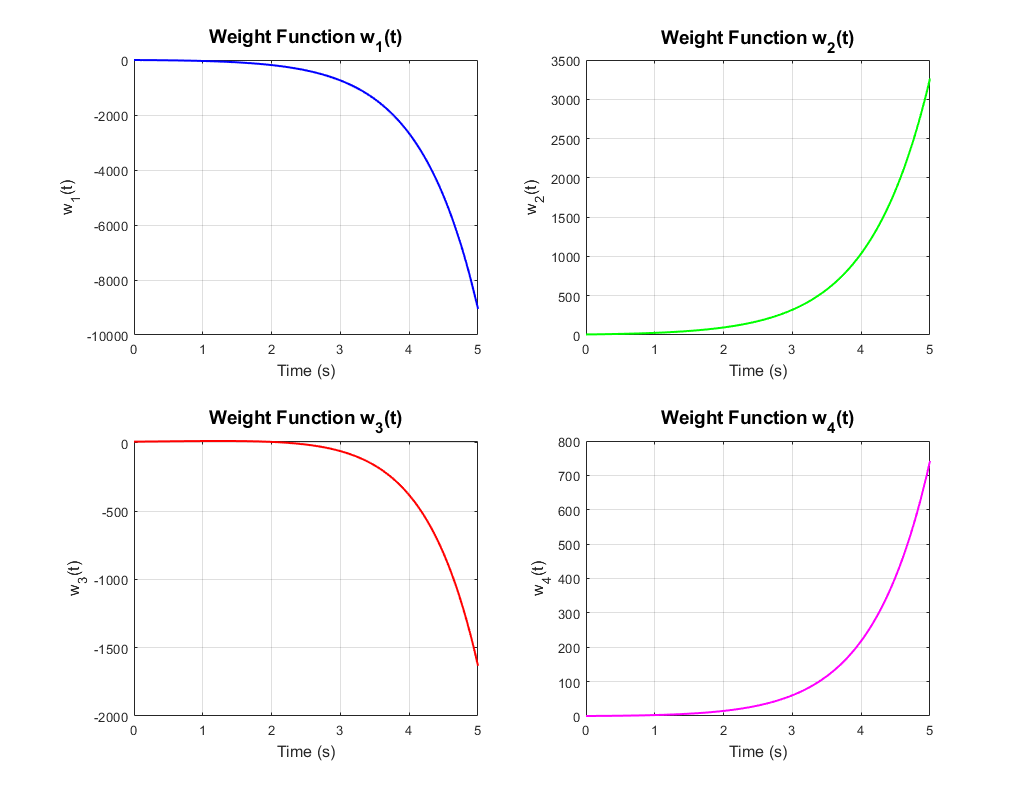
\includegraphics[scale=0.585]{1task_wi.png}
        \captionsetup{skip=0pt}
        \caption{Графики весовых функций $w_i(t)$}
        \label{fig:1task_wi}
    \end{figure}
    \begin{figure}[H]
        \centering
        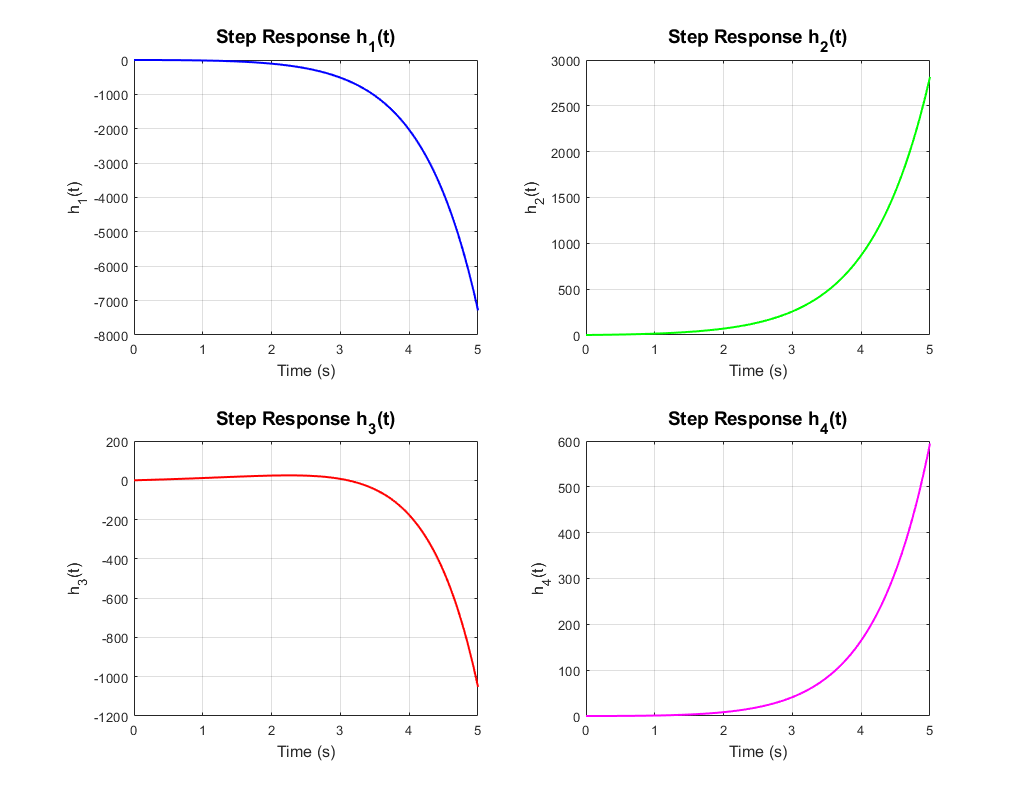
\includegraphics[scale=0.585]{1task_hi.png}
        \captionsetup{skip=0pt}
        \caption{Графики переходных функций $h_i(t)$}
        \label{fig:1task_hi}
    \end{figure}


    \subsection{Частотные характеристики системы}
    Выведем аналитические выражения частотных характеристик системы,
    таких как АЧХ, ФЧХ, ЛАЧХ, ЛФЧХ. АЧХ находим по формуле
    $$
    A_k(\omega)=|W_{n,m}(i\omega)|=\sqrt{\text{Re}^2\left\{ W_{n,m}(i\omega)\right\}+\text{Im}^2\left\{ W_{n,m}(i\omega) \right\}}
    $$
    Найдем $A_1(\omega)$
    $$
    A_1\left( \omega \right)=|W_{1,1}(i\omega)|=\bigg|\dfrac{-i\omega-11}{(i\omega-1)^2}\bigg|
    $$
    ФЧХ ищется по формуле
    $$
    \varphi_k=\text{atan2}\left( \text{Im}\left\{ W_{n,m}(i\omega) \right\}, \text{Re}\left\{ W_{n,m}(i\omega)\right\}\right)
    $$


    \section{Приложение А}
    \begin{lstlisting}[label=task1, caption={Программа для задания 1}]
        tbd
    \end{lstlisting}
\end{document}